\setchapterpreamble[u]{\margintoc}
\chapter{Intepolazione}
\labch{interp}


\section{Implementazione preliminaria}

Prima di procedere è necessario specificare varie funzioni/classi appositamente create
per la scrittura del codice e una più facile implementazione degli algoritmi.

\paragraph{Classe \texttt{FunctionData}}

La classe \texttt{FunctionData} ha lo scopo di conservare i dati numerici ottenuti
dalla computazione delle varie funzioni (in questo modulo principalmente polinomi) \sidenote{Nell'implementazione della classe
	può essere trovata anche un'implementazione apposita di un iterator per
	facilitare l'utilizzo dei valori quando ciclati.}.

Essa ha come membri due vettori di tipo \texttt{std::vector} che conservano le
informazioni di $x$ e $f(x)$.

\paragraph{Classe \texttt{Range}}

La classe \texttt{Range} ha invece lo scopo di rappresentare una successione di
punti $\left\{a_i\right\}_{i \in (a, b) \subset \mathbb{R}}$ (la rappresentazione
prevede intervalli inclusivi ed esclusivi).

Scopo principale della classe sarà quello di generare nodi di distanza finita e
nodi di Chebyshev.

\textit{Ulteriori informazioni sulle due classi possono essere trovate nella
	documentazione dedicata negli appositi header} \texttt{function\_data.hpp} \textit{e}
\texttt{range.hpp}.

\section{Esercizi}

\subsection{Esercizio 6}

\paragraph{Nozioni teoriche}

Il metodo più semplice per ottenere il polinomio di interpolazione è quello di ottenere

% TODO:

\paragraph{Implementazione metodo diretto}

\subparagraph{File necessari} \texttt{interpolation.hpp}

Come primo step si ottiene la matrice di Vandermonde dalla sua definizione:

\begin{lstlisting} [language=C++]

// "values" sono i valori {x_1, x_2, ...} da inserire 
template <typename T>
tensor::Tensor<T> VandermondeMatrix(std::vector<T> const &values) {
  auto mat = tensor::Tensor<T>::SMatrix(values.size());

  for (int i = 0; i < values.size(); i++) {
    for (int j = 0; j < values.size(); j++) {
      mat(i, j) = pow(values[i], j);
    }
  }

  return mat;
}
    
\end{lstlisting}

Successivamente si risolve il sistema lineare utilizzando il metodo di Gauss
(invertire la matrice necessiterebbe di un ulteriore eliminazione di Gauss ed
ulteriore allocamento di memoria).

\begin{lstlisting} [language=C++]
template <typename T>
std::vector<T> DirectCoefficients(func::FunctionData<T> const &f) {
  auto f_tensor = tensor::Tensor<T>::FromData(f.F());

  tensor::Tensor<T> vande_matrix = VandermondeMatrix(f.X());
  tensor::Tensor<T> values =
      tensor::GaussianElimination(vande_matrix, f_tensor);

  // Trasforma l'oggetto tensore in std::vector
  return values.RawData();
}

\end{lstlisting}

\paragraph{Implementazione metodo di Newton}

Analogamente al metodo diretto calcoliamo i coefficienti per il polinomio di
Newton seguendo la formula citata precedentemente otteniamo.

\begin{lstlisting} [language=C++]
template <typename T>
std::vector<T> NewtonCoefficients(func::FunctionData<T> const &f) {
  int N = f.Size();

  std::vector<T> a(N);

  auto A = tensor::Tensor<double>::SMatrix(N);

  // Rempiamo la prima colonna con i valori della funzione
  for (int i = 0; i < N; i++) {
    A(i, 0) = f.F(i);
  }

  // Calcoliamo le differenze divise
  for (int j = 1; j < N; j++) {
    for (int i = 0; i < N - j; i++) {
      A(i, j) = (A(i + 1, j - 1) - A(i, j - 1)) / (f.X(i + j) - f.X(i));
    }
  }

  // Estrapoliamo i coefficienti
  for (int i = 0; i < N; i++) {
    a[i] = A(0, i);
  }

  return a;
}
\end{lstlisting}

\subparagraph{Considerazioni} L'algoritmo è direttamente implementato rispetto a
lla logica che abbiamo considerato per calcolare i coefficienti di Newton.
Uno svantaggio di questo algoritmo sta nell utilizzo dell'oggetto Tensor, infatti
il funzionamento interno della classe traduce una matrice 2x2 in una vettore
contiguo: questo permette un ottimizzazzione della cache della cpu rispetto ad un
vettore di vettori, ma nel caso utilizzato la matrice è solo occupata a metà,
lasciando inizializzati a 0 molti valori non utilizzati nella computazione dei
coefficient.
Un modo per evitare ciò sarebbe per esempio quello di implementare un oggetto ad hoc
per il problema, ai fini concettuali, però, l'implementazione sarebbe la medesima.

\subsubsection{Punto 1}

\paragraph{Analisi e conclusioni}

\begin{marginfigure}
	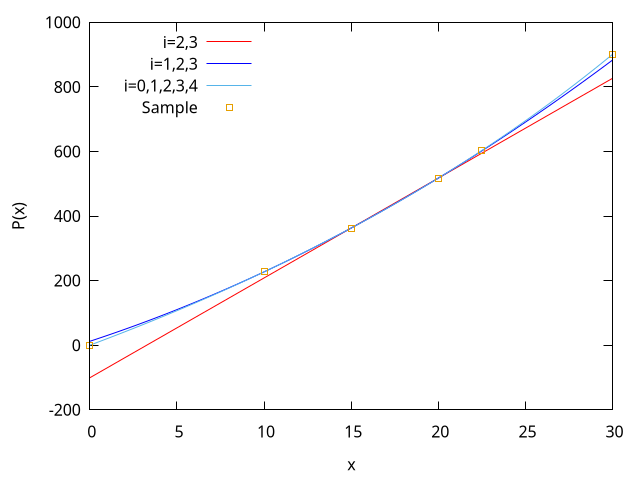
\includegraphics[width=1.5\textwidth]{newton_all.png}
	\caption{Confronto tra i vari sample}
	\label{fig:newton}
\end{marginfigure}

Dalla implementazione dei metodi sopra citati e dai dati forniti dal problema
otteniamo la figura \reffig{newton}.

Come si puo' notare il polinomio di Newton nel caso (1) e (2) non attraversa il punto $x_5$, poiche' esso garantisce solamente di passare esattamente nei punti
dati inizialmente. Il caso(3) e' invece un caso particolare, infatti, sembra che il polinomio di Newton passi esattamette per $x_5$ (almeno entro l'errore in doppia precisione), questo puo' essere spiegato se il polinomio coincide
esattamente con la funzione campionata oppure in generale per altri casi specifici
altamente non banali. (per esempio, la funzione e' tale che la sua espansione in serie coincida in quel
punto con il polinomio di newton).

\subsubsection{Punto 2: Funzione di Runge}

\paragraph{Analisi dei risultati}

\begin{marginfigure}
	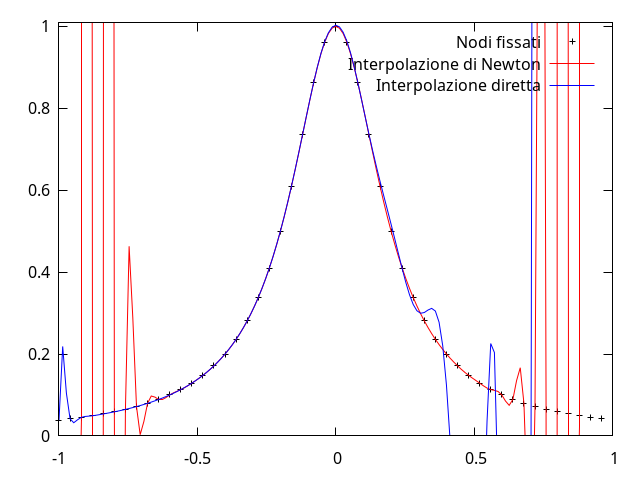
\includegraphics[width=1.5\textwidth]{interp_fixed.png}
	\caption{Nodi equidistanti}
	\label{fig:runge_fixed}
\end{marginfigure}

\begin{marginfigure}
	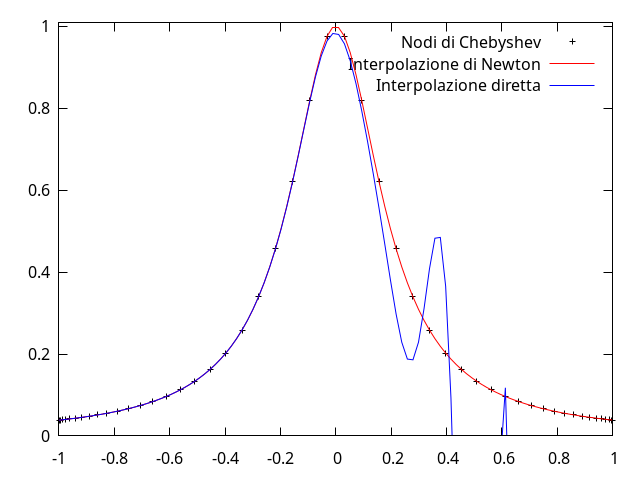
\includegraphics[width=1.5\textwidth]{interp_chebyshev.png}
	\caption{Nodi di Chebyshev}
	\label{fig:runge_chebyshev}
\end{marginfigure}

Dalla \reffig{runge_fixed} si puo' osservare il fenomeno di Runge, il
carattere oscillatorio si presenta in entrambi i metodi: nel metodo di Newton si
osserva un carattere oscillatorio piu' accentuato rispetto al metodo diretto, questo e' dovuto al fatto che il metodo di Newton e' un metodo iterativo che tende a convergere al polinomio di interpolazione, mentre nel metodo diretto il problema
e' meno notevole. %TODO: verificare

Attraverso l'utilizzo dei nodi di Chebyshev si evince (\reffig{runge_chebyshev}) che il problema presentatosi precedentemente e' risolto, si nota ancora piu' chiaramente anche che il metodo diretto dopo circa $x=0$ diventa \textit{ill-conditioned}: il vantaggio ottenuto nel caso dei nodi fissi (per valori inferiori a 0) dal metodo diretto
e' completamente superato dal metodo di Newton con il nuovo campionamento.

\paragraph{Conclusioni}

Durante il campionamento di una funzione e' di fondamentale importanza la scelta
dei nodi ed il metodo utilizzato: i risultati ottenuti, infatti, possono variare
drasticamente.


\subsection{Esercizio 7}

\paragraph{Nozioni teoriche}

Un'ulteriore via per interpolare una funzione e' di non considerare un interpolazione globale, ma una locale tra i punti di campionamento vicini. Si puo' quindi
decidere di utilizzare una funzione linare, quadratica, \dots per unire i vari
punti, il metodo viene chiamato Spline.

%TODO: Aggiungere tutta la teoria?

\paragraph{Implementazione}

L'implementazione di un algoritmo di grado $n$ segue in modo induttivo dai casi
di $n=1,2,3, \dots$: si impongono continuita' delle derivate e valori ai parametri liberi (per esempio si impone che la derivata sia nulla nel caso quadratico).

Nel caso $n=1,2$ svolto l'algoritmo generale non e' strettamente necessario e si
possono riempire direttamente le matrici ottenute nelle note, in caso di n piu'
grandi una ristrutturazione del codice sarebbe necessaria.

Per completezza si include di seguito l'algoritmo generale:

\begin{algorithm}
	\For{$i=0; i < n$}
	{
		\For{$a=0; a < q$}
		{
			$M_{iq, iq+a} \leftarrow (x_i)^a$ \\
			$M_{iq+1, iq+a} \leftarrow a(x_i)^{a-1}$\quad \textit{Imponiamo la continuita' della derivata prima}
		}
		$b_i \leftarrow f_i$ \\
		$b_{i+1} \leftarrow 0$ \quad \textit{Prendiamo come convenzione 0}
	}
	\If{$q>2$} {
		\For{$i=0; i < n-1$}
		{
			\For{$a=1; a < q$}
			{
				\textit{Condizione di continuita' tra le derivate di ordine superiore} \\
				$M_{iq+2, iq+a} \leftarrow a(x_{i+1})^{a-1}$ \\
				$M_{iq+2,(i+1)q+a} \leftarrow -a(x_{i+1})^{a-1}$
			}
		}
	}
\end{algorithm}

\paragraph{Analisi risultati}

\begin{marginfigure}
    \hspace{-2.1cm}
	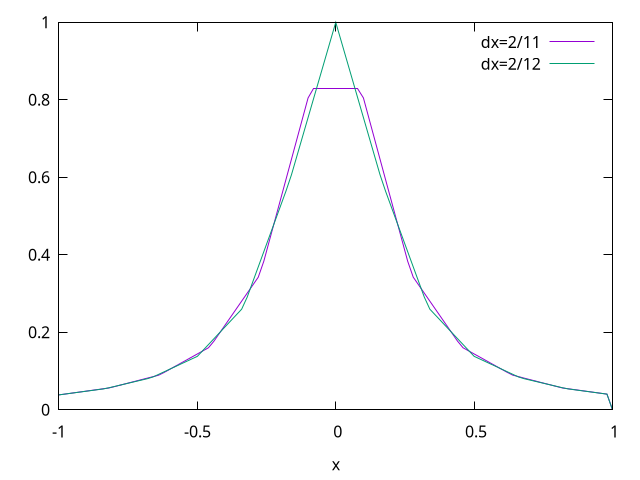
\includegraphics[width=1.5\textwidth]{linear_spline.png}
	\caption{Spline lineare}
	\label{fig:linear_spline}
\end{marginfigure}

\begin{marginfigure}
    \hspace{-2.1cm}
	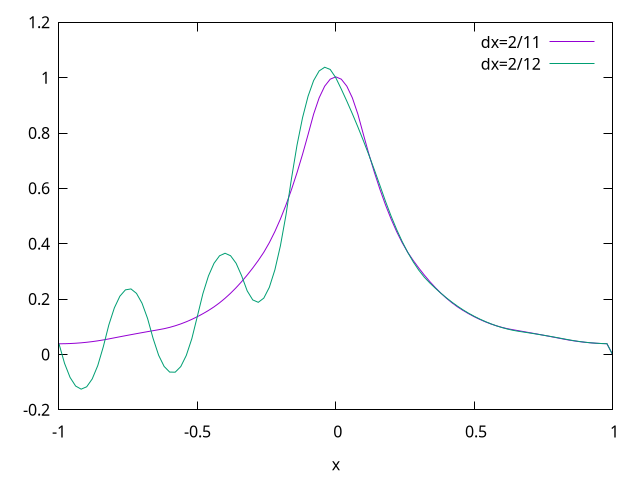
\includegraphics[width=1.5\textwidth]{quad_spline.png}
	\caption{Spline quadratica}
	\label{fig:quad_spline}
\end{marginfigure}

\subparagraph{Spline lineare}
L'analisi di \reffig{linear_spline} e' triviale: la spline lineare unisce semplicemente i punti campionati, la differenza sta quindi nel fatto che nei differenti
step di campionamento; in un caso si campiona 0 ma non nell'altro caso.

\subparagraph{Spline quadratica}

Il caso in \reffig{quad_spline} e' molto piu' particolare, la differenza di campionamento, infatti, causa l'emergere di un carattere oscillatorio nella interpolazione. La spiegazione e' facilmente intuibile se si guarda l'interpolazione da destra verso sinistra: dovendo passare per $(0,1)$ e dovendo valere $S'_{x_i}=S'_{x_{i+1}}=0$ allora la spline sovrastima il valore di $f(0)$. Questo fenomeno e' noto come \textit{overshooting}.
La \textit{sovrastima} causa nei punti successivi (che devono soddisfare le regole precedenti e quindi devono passare per i punti di campionamento) all'andamento osservato. Questo non si verifica nel primo campionamento poiche' viene mantenuta la simmetria della funzione.


